%%%%%%%%%%%%%%%%%%%%%%%%%
% Dokumentinformationen %
%%%%%%%%%%%%%%%%%%%%%%%%%
\newcommand{\titleinfo}{Geotechnik Zusammenfassung HS17}
\newcommand{\authorname}{\href{mailto:noelle.egger@hsr.ch}{No\"elle Egger}}
\newcommand{\authoremail}{\href{mailto:noelle.egger@hsr.ch}{noelle.egger@hsr.ch}}
\newcommand{\versioninfo}{$ V0.1 $}

%%%%%%%%%%%%%%%%%%%%%%%%%%%%%%%%%%%%%%%%%%%%%
% Standard projektübergreifender Header für 
% - Makros 
% - Farben
% - Mathematische Operatoren
%
% dORT NUR ERGÄNZEN, NICHTS LÖSCHEN
%%%%%%%%%%%%%%%%%%%%%%%%%%%%%%%%%%%%%%%%%%%%%
%BuG-Fix
%Package pdf Error: Driver file ................ not found
%If you have a luatex driver fail uncomment these lines
\RequirePackage{luatex85}
\def\pgfsysdriver{pgfsys-pdftex.def}

% Genereller Header
\documentclass[11pt,twoside,a4paper,fleqn]{article}
% Dateiencoding
\usepackage[utf8]{inputenc}
\usepackage[T1]{fontenc}	%ä,ü...
% Seitenränder
\usepackage[left=1cm,right=1cm,top=0.5cm,bottom=0.5cm,includeheadfoot]{geometry}
% Sprachpaket 
\usepackage[english, ngerman]{babel} % Silbentrennung und Rechtschreibung Englisch und Deutsch

%%%%%%%%%%%%%%%%%%%%%%%
%% Wichtige Packages %%
%%%%%%%%%%%%%%%%%%%%%%%
\usepackage{amsmath}                % Allgemeine Matheumgebungen									
\usepackage{amssymb}                % Fonts: msam,msbm, eufm & Mathesymbole, Mengen (lädt automatisch amsfonts)									
\usepackage{array}                  % \newcolumntype, \firsthline, ,\lasthline, m{width}, b{width}									
\usepackage{caption}                % Bildunterschriften									
\usepackage{enumitem}               % basic environments: enumerate, itemize, description									
\usepackage{fancybox}               % \fbox: \shad­ow­box, \dou­ble­box, \oval­box, \Oval­box									
\usepackage{fancyhdr}               % Seiten schöner gestalten, insbesondere Kopf- und Fußzeile									
\usepackage{floatflt}               % Textumflossene Abbildungen \begin{floatingfigure}[r]{Breite} : r rechts, l links, p links auf geraden Seiten und rechts auf ungeraden Seiten								
\usepackage{graphicx}               % \includegraphics[keyvals]{imagefile}, [draft]graphicx zeigt nur Namen und Rahmen an, [final] hebt diese option auf => Bild wird angezeigt    									
\usepackage{hyperref}               % Erstellt Verweise innerhalb und nach außerhalb eines PDF Dokumentes.									
\usepackage{lastpage}               % Bspw. : Page 1 of 3 => \thepage\ of \pageref{LastPage}									
\usepackage{listings}               % Erlaubt es Programmcode in der gewünschten Sprache zu hinterlegen (C++, Matlab,..). Definition der Sprache mit \lstset{language=name}..									
\usepackage{longtable}              % Longtable erlaubt es Tabellen zu erstellen die bei der nächsten Seite weiterlaufen. (Bricht automatisch um)									
\usepackage{mathabx}                % Mathesymbole									
\usepackage{mathrsfs}               % \mathscr (Benötigt für Fourierreihen-Symbol)									
%\usepackage{mathtools}              % Extension package to amsmath									
\usepackage{multicol}               % multicols-Umgebung \begin{multicols}{3} erzeugt Abschnitt mit 3 Spalten									
\usepackage{multirow}               % Tabelle: ermöglicht es Felder mehrerer Zeilen in einem zusammenzufassen									
\usepackage{pdflscape}              % adds PDF support to the environment 'landscape'									
\usepackage{pxfonts}                % Symbole, griechisches Alphabet, Integrale...									
\usepackage{rotating}               % sideways, turn{degree}, rotate{degree}, sidewaysfigure, sidewaystable Umgebung									
\usepackage{subcaption}             % Bildunterschriften für Subfigures									
\usepackage{tabularx}               % tabularx-Umgebung: Hat feste Gesamtbreite, \begin{tabularx}{\textwidth}{c c c c c} X: Spalte mit variabler Breite, l, c, r, p{breite}, m{breite}									
\usepackage{textcomp}               % text symbols: baht, bullet, copyright, musical-note, onequarter, section, yen									
\usepackage{tikz}                   % Tikz Umgebung zur Grafikerzeugung									
\usepackage{titlesec}               % Überschriften zu Textabstände
\usepackage{trfsigns}               % Transformationszeichen \laplace, \Laplace..									
\usepackage{trsym}                  % Weitere Laplace Zeichen erlaubt auch vertikale Transformationszeichen									
\usepackage{verbatim}               % verbatim, verbatim*, comment Umgebung									
\usepackage{wrapfig}                % Textumflossene Bilder und Tabellen, \begin{wrapfigure}[Zeilen]{Position}[Ueberhang]{Breite}									
\usepackage{xcolor}                 % \pagecolor{color}, \textcolor{color}{text}, \colorbox{color}{text}, \fcolorbox{border-color}{fill-color}{text}									
\usepackage{titlesec}
% Zum Bilder einfach in Tabellen einfügen (valign=t)
\usepackage[export]{adjustbox}

%%%%%%%%%%%%%%%%%%%%
% Generelle Makros %
%%%%%%%%%%%%%%%%%%%%
\newcommand{\skript}[1]{$_{\textcolor{red}{\mbox{\small{Skript S.#1}}}}$}
\newcommand{\verweis}[2]{\small{(siehe auch \ref{#1}, #2 (S. \pageref{#1}))}}
\newcommand{\verweiskurz}[1]{(\small{siehe \ref{#1}\normalsize)}}
\newcommand{\subsubadd}[1]{\textcolor{black}{\mbox{#1}}}
\newcommand{\formelbuch}[1]{$_{\textcolor{red}{\mbox{\small{S#1}}}}$}

\newcommand{\kuchling}[1]{$_{\textcolor{red}{\mbox{\small{Kuchling #1}}}}$}
\newcommand{\stoecker}[1]{$_{\textcolor{grey}{\mbox{\small{Stöcker #1}}}}$}
\newcommand{\sachs}[1]{$_{\textcolor{blue}{\mbox{\small{Sachs S. #1}}}}$}
\newcommand{\hartl}[1]{$_{\textcolor{green}{\mbox{\small{Hartl S. #1}}}}$}

\newcommand{\schaum}[1]{\tiny Schaum S. #1}

\newcommand{\skriptsection}[2]{\section{#1 {\tiny Skript S. #2}}}
\newcommand{\skriptsubsection}[2]{\subsection{#1 {\tiny Skript S. #2}}}
\newcommand{\skriptsubsubsection}[2]{\subsubsection{#1 {\tiny Skript S. #2}}}

\newcommand{\matlab}[1]{\footnotesize{(Matlab: \texttt{#1})}\normalsize{}}

% Syntax: \bmu{Pfad zum Bild}{Bildgrösse}{Beschriftung des Bildes}
\newcommand{\bl}[2]{
	\begin{figure}[h]
		\flushleft  % linksbuendig
		\includegraphics[width=#1]{#2} \\
	\end{figure}
}
\newcommand{\br}[2]{
	\begin{figure}[h]
		\flushright  % rechtsbuendig
		\includegraphics[width=#1]{#2} \\
	\end{figure}
}

\newcommand{\bild}[2]{
	\begin{figure}[h]
		\centering  % zentriert
		\includegraphics[width=#1]{#2} \\
	\end{figure}
}

\newcommand\tabbild[2][]{%
	\raisebox{0pt}[\dimexpr\totalheight+\dp\strutbox\relax][\dp\strutbox]{%
		\includegraphics[#1]{#2}%
	}%
}

\newcolumntype{P}[1]{>{\raggedright\arraybackslash}p{#1}} %Tabelle linksausgerichtet
\newcolumntype{L}[1]{>{\raggedleft\arraybackslash}p{#1}} %Tabelle rechtsausgerichtet
\newcolumntype{C}[1]{>{\centering\arraybackslash}p{#1}}



%%%%%%%%%%
% Farben %
%%%%%%%%%%
\definecolor{black}{rgb}{0,0,0}
\definecolor{red}{rgb}{1,0,0}
\definecolor{white}{rgb}{1,1,1}
\definecolor{grey}{rgb}{0.8,0.8,0.8}
\definecolor{green}{rgb}{0,.8,0.05}
\definecolor{brown}{rgb}{0.603,0,0}
\definecolor{mymauve}{rgb}{0.58,0,0.82}


%%%%%%%%%%%%%%%%%%%%%%%%%%%%
% Mathematische Operatoren %
%%%%%%%%%%%%%%%%%%%%%%%%%%%%
\DeclareMathOperator{\sinc}{sinc}
\DeclareMathOperator{\sgn}{sgn}
\DeclareMathOperator{\Real}{Re}
\DeclareMathOperator{\Imag}{Im}
%\DeclareMathOperator{\e}{e}
\DeclareMathOperator{\cov}{cov}
\DeclareMathOperator{\PolyGrad}{PolyGrad}

%Grösse Integral anpassen
\def\Int{\mbox{\Large$\displaystyle\int$\normalsize}}
\def\OInt{\mbox{\Large$\displaystyle\oint$\normalsize}}

%Makro für 'd' von Integral- und Differentialgleichungen 
\newcommand*{\diff}{\mathop{}\!\mathrm{d}}

%%%%%%%%%%%%%%%%%%%%%%%%%%%
% Fouriertransformationen %
%%%%%%%%%%%%%%%%%%%%%%%%%%%

% Fouriertransformationen
\unitlength1cm
\newcommand{\FT}
{
	\begin{picture}(1,0.5)
	\put(0.2,0.1){\circle{0.14}}\put(0.27,0.1){\line(1,0){0.5}}\put(0.77,0.1){\circle*{0.14}}
	\end{picture}
}


\newcommand{\IFT}
{
	\begin{picture}(1,0.5)
	\put(0.2,0.1){\circle*{0.14}}\put(0.27,0.1){\line(1,0){0.45}}\put(0.77,0.1){\circle{0.14}}
	\end{picture}
}


%%%%%%%%%%%%%%%%%%%%%%%%%%%%
% Allgemeine Einstellungen %
%%%%%%%%%%%%%%%%%%%%%%%%%%%%

\setitemize{noitemsep,topsep=0pt,parsep=0pt,partopsep=0pt} %kompakte itemize
\setenumerate{noitemsep,topsep=0pt,parsep=0pt,partopsep=0pt} %kompakte enumerate

%Pdf Info
\hypersetup{pdfauthor={\authorname},pdftitle={\titleinfo},colorlinks=false}
\author{\authorname}
\title{\titleinfo}

% Abstände Text zu Übertiteln / Einzug
\titlespacing{\section}{12pt}{1em}{0.5em}
\titlespacing{\subsection}{12pt}{1em}{0.5em}
\titlespacing{\subsubsection}{12pt}{1em}{0.5em}

%%%%%%%%%%%%%%%%%%%%%%%
% Kopf- und Fusszeile %
%%%%%%%%%%%%%%%%%%%%%%%
\pagestyle{fancy}
\fancyhf{}
%Linien oben und unten
\renewcommand{\headrulewidth}{0.5pt} 
\renewcommand{\footrulewidth}{0.5pt}

%Kopfzeile links bzw innen
\fancyhead[L]{\titleinfo{ }\tiny{(\versioninfo)}}
%Kopfzeile mitte
%\fancyhead[C]{}
%Kopfzeile rechts bzw. aussen
\fancyhead[R]{Seite \thepage { }von \pageref{LastPage}}

%Fusszeile links bzw. innen
\fancyfoot[L]{\footnotesize{\authorname}}
%Fusszeile mitte
%\fancyfoot[C]{\footnotesize{\authoremail}}
%Fusszeile rechts bzw. ausen
\fancyfoot[R]{\footnotesize{\today}}
% Einrücken verhindern versuchen
\setlength{\parindent}{0pt}

%%%%%%%%%%%%%%%%%%%%%%%%%%%%%%%%%%%%%%%
%% Makros & anderer Low-Level bastel %%
%%%%%%%%%%%%%%%%%%%%%%%%%%%%%%%%%%%%%%%
% Zeilenhöhe Tabellen:
\newcommand{\arraystretchOriginal}{1.5}
\renewcommand{\arraystretch}{\arraystretchOriginal}

\makeatletter
%% Makros für den Arraystretch (bei uns meist in Tabellen genutzt, welche Formeln enthalten)
% Default Value
\def\@ArrayStretchDefault{1} % Entspricht der Voreinstellung von Latex

% Setzt einen neuen Wert für den arraystretch
\newcommand{\setArrayStretch}[1]{\renewcommand{\arraystretch}{#1}}

% Setzt den arraystretch zurück auf den default wert
\newcommand{\resetArrayStretch}{\renewcommand{\arraystretch}{\@ArrayStretchDefault}}

% Makro zum setzten des Default arraystretch. Kann nur in der Präambel verwendet werden.
\newcommand{\setDefaultArrayStretch}[1]{%
    \AtBeginDocument{%
        \def\@ArrayStretchDefault{#1}
        \renewcommand{\arraystretch}{#1}
    }
}
\makeatother

%% Achtung Symbol \danger
\newcommand*{\TakeFourierOrnament}[1]{{%
        \fontencoding{U}\fontfamily{futs}\selectfont\char#1}}
\newcommand*{\danger}{\TakeFourierOrnament{66}}
%%%%%%%%%%%%%%%%
% Code Layout %
%https://en.wikibooks.org/wiki/LaTeX/Source_Code_Listings
%%%%%%%%%%%%%%%

\definecolor{mygreen}{rgb}{0,0.6,0}
\definecolor{mygray}{rgb}{0.5,0.5,0.5}
\definecolor{mymauve}{rgb}{0.58,0,0.82}

\lstset{ %
    firstnumber=1,
    backgroundcolor=\color{white},   % choose the background color; you must add        \usepackage{color} or \usepackage{xcolor}
    basicstyle=\footnotesize\ttfamily, % the size of the fonts that are used for the code
    breakatwhitespace=false,         % sets if automatic breaks should only happen at whitespace
    breaklines=true,                 % sets automatic line breaking
    captionpos=b,                    % sets the caption-position to bottom
    commentstyle=\color{mygreen},    % comment style
    deletekeywords={...},            % if you want to delete keywords from the given language
    otherkeywords={...},             % if you want to add more keywords to the set
    escapeinside={\%*}{*\%},          % if you want to add LaTeX within your code
    extendedchars=true,              % lets you use non-ASCII characters; for 8-bits encodings only, does not work with UTF-8
    frame=single,	                 % adds a frame around the code
    keepspaces=true,                 % keeps spaces in text, useful for keeping indentation of code (possibly needs columns=flexible)
    keywordstyle=\color{blue},       % keyword style
    language=C++,                    % the language of the code   
    numbers=left,                    % where to put the line-numbers; possible values are (none, left, right)
    numbersep=5pt,                   % how far the line-numbers are from the code
    numberstyle=\tiny\color{mygray}, % the style that is used for the line-numbers
    rulecolor=\color{black},         % if not set, the frame-color may be changed on line-breaks within not-black text (e.g. comments (green here))
    showspaces=false,                % show spaces everywhere adding particular underscores; it overrides 'showstringspaces'
    showstringspaces=false,          % underline spaces within strings only
    showtabs=false,                  % show tabs within strings adding particular underscores
    stepnumber=2,                    % the step between two line-numbers. If it's 1, each line will be numbered
    stringstyle=\color{mymauve},     % string literal style
    tabsize=2,	                     % sets default tabsize to 2 spaces
    %title=\lstname                   % show the filename of files included with         \lstinputlisting; also try caption instead of title
}

\lstdefinestyle{customc++}{
    belowcaptionskip=1\baselineskip,
    %frame=L,
    xleftmargin=\parindent,
    language=C++,
    keywordstyle=\bfseries\color{blue},
    commentstyle=\itshape\color{mygreen},
    identifierstyle=\color{black},
    stringstyle=\color{gray},
}

\lstdefinestyle{cppunit}{
    belowcaptionskip=1\baselineskip,
    %frame=L,
    xleftmargin=\parindent,
    language=C++,
    keywordstyle=\bfseries\color{blue},
    keywordstyle=[2]\bf\color{black}, %not sure why \bf works, but it does
    commentstyle=\itshape\color{mygreen},
    identifierstyle=\color{black},
    stringstyle=\color{gray},
    keywords=[2]{  %Cpp Unit Keywords
        CPPUNIT_ASSERT,
        CPPUNIT_TEST,
        CPPUNIT_TEST_EXCEPTION,
        CPPUNIT_TEST_END,
        CPPUNIT_TEST_SUITE,
        CPPUNIT_TEST_SUITE_REGISTRATION,
        CPPUNIT_TEST_SUITE_END},
}

\lstdefinestyle{cppqt}{
    belowcaptionskip=1\baselineskip,
    %frame=L,
    xleftmargin=\parindent,
    language=C++,
    keywordstyle=\bfseries\color{blue},
    keywordstyle=[2]\bfseries\color{red},
    commentstyle=\itshape\color{mygreen},
    identifierstyle=\color{black},
    stringstyle=\color{gray},
    keywords=[2]{           % qt-Keywords
		Qt,
        SIGNAL,
        SLOT,
        QApplication,
        QDialog,
        QGridLayout,
        QPushButton,
        QLabel,
        QVBoxLayout,
        QHBoxLayout,
        QWidget,
        QGroupBox,
        QFont,
        QLineEdit,
        QRadioButton,
        QPen,
        QRect,
        QPaintEvent,
        QBrush,
        QPixmap,
        QPainter,
        QString,
        QPoint,
        update()},
}

\lstdefinestyle{cdoxy}{
    belowcaptionskip=1\baselineskip,
    %frame=L,
    xleftmargin=\parindent,
    language=C++,  
    keywordstyle=\bfseries\color{blue},
    commentstyle=\itshape\color{mygreen},
    identifierstyle=\color{black},
    stringstyle=\color{gray},
    otherkeywords={           % DoxygenKeywords
        ...,
        ....,
        @mainpage,
        @file,
        @author,
        @version,
        @date,
        @bug,
        @brief,
        @extended,
        @param,
        @return,
        @warning,
        @note,
        @see},
}

%choose customstyle in DOC with \lstinputlisting[style=custom]{path}
\lstset{style=customc++}

% Möglichst keine Ergänzungen hier, sondern in header.tex

%%%%%%%%%%%%%%%%%%%%%%%%%%%%%%%%%%%%%%%%%%%%%%%%%%%%%%%%%%%%%%%%%%%%%%%%%%%%%%%%%%%%%%%%%%%%%%%%
%%%%%%%%%%%%%%%%%%%%%%%%%%%%%%%%%%%%%%%%%%%%%%%%%%%%%%%%%%%%%%%%%%%%%%%%%%%%%%%%%%%%%%%%%%%%%%%%

\begin{document}
\maketitle
\tableofcontents
\thispagestyle{empty}
\newpage
\section{Konsolidation}
%\begin{minipage}{0.5\linewidth}
%	\renewcommand{\arraystretch}{2}
%\begin{alignat*}{2}
%	\text{Dehnung} 		& \qquad	&  \epsilon &= \frac{\Delta h}{h_0}  \\
%	\text{Porenziffer}  &&  e_0 		&= \frac{\gamma_s}{\gamma_d} -1  \\
%						&&  e 			&=e_0-\epsilon \cdot \left(1+ e_0\right) \\
%	&\rightarrow&  \frac{\Delta h}{h} 	&= \frac{e_0 - e}{1+e_0} 	\\		
%	&\rightarrow& \Delta h 				&= \frac{\Delta \sigma \cdot h_0}{M_E} \\
%	M_E-Modul	&&  M_E					&=\frac{\Delta \sigma}{\Delta \epsilon}=\frac{1+e_0}{C_c \cdot 0.434}\cdot\sigma_m \\	
%	&\rightarrow &  \gamma_d			&=\frac{\gamma}{1+w} \\
%				&& n&=\frac{\gamma-\gamma_d}{S_r\cdot\gamma_w} \\
%				&& e_0&=\frac{n}{1-n} \\
%				&& \gamma&=\frac{G}{V}\cdot g \\
%				&& \gamma_s&=16-17 \; kN/m^3 \\
%	\rightarrow Oedometer && \sigma&=M_E \cdot \epsilon \\
%				& \rightarrow& M_E&\neq E, \hspace{0.25cm}\text{da} \hspace{.25cm} \epsilon_2=\epsilon_3=0 \\
%				&& \sigma_m&=\frac{2\cdot\sigma_0+\Delta \sigma}{2} \\
%	Konsolidationskoeffizient [cm^2/s]&&  C_v&=\frac{M_E\cdot k}{\gamma_w}=\frac{T_v\cdot d^2}{t} \\
%	\text{Durchlässigkeitswert} && k&=\frac{C_v\cdot\gamma_w}{M_E} \\
%	Zeitfaktor	&& T_V&=\frac{t\cdot C_V}{d^2}=\frac{t\cdot M_E\cdot k}{\gamma_w\cdot d^2} \\
%\end{alignat*}
%\renewcommand{\arraystretch}{\arraystretchOriginal}
%\end{minipage}
%
%\begin{minipage}{0.5\linewidth}
%	\renewcommand{\arraystretch}{2}
%\begin{alignat*}{2}
%		Einheiten	&\qquad&\\
%		M_E			&& \left[\frac{kN}{m^2}\right]\\
%		\gamma		&& [\frac{kN}{m^3}]\\
%		\sigma		&& [\frac{kN}{m^2}]\\
%		C_v			&& [\frac{m^2}{s}]\\
%		Umrechnung	&& \gamma_w&=\frac{kN}{m^3}\cdot 10^{-6}=\frac{kN}{cm^3} \\
%		&&M_E&=\frac{kN}{m^2}\cdot 10^{-4}=\frac{kN}{cm^2}	\\
%\end{alignat*}
%\renewcommand{\arraystretch}{\arraystretchOriginal}
%\end{minipage}
%
%\begin{itemize}
%	\item hh
%	\item hh
%	\begin{itemize}
%		\item hh
%		\item hh
%		\[ \gamma_s=16-17 \hspace{2cm} \left[\frac{kN}{m^3}\right] \]
%	\end{itemize}
%\end{itemize}
	\begin{minipage}[t]{0.25\linewidth}
	\subsection{Umrechnungen}
	\begin{tabular}{|l|l|}
	\hline
	kPa 				& $\frac{kN}{m^2}$ \\ \hline
	Pa					& $\frac{N}{m^2}$  \\ \hline
	$\frac{kN}{m^2}$	& $\frac{N}{mm}$	\\ \hline
	$\gamma_w=\frac{kN}{m^3}\cdot 10^{-6}$ & $\frac{kN}{cm^3}$ \\ \hline
	$M_E=\frac{kN}{m^2}\cdot 10^{-4}$ & $\frac{kN}{cm^2}$	\\ \hline
	\end{tabular}
\end{minipage}
\begin{minipage}[t]{0.5\linewidth}
	\subsection{Materialverhalten mit Oedometer}

	\begin{tabular}{l|l|l}
				& Formeln 									& Einheiten \\ \hline \hline
	
		Dehnung &$\epsilon = \frac{\Delta h}{h_0}$& \\ \hline
	
		Porenziffer&$\e_0=\frac{\gamma_s}{\gamma_d} -1$		& \\
				&$e=e_0-\epsilon \cdot \left(1+ e_0\right)$	&\\
				&$\rightarrow\frac{\Delta h}{h}=\frac{e_0 - e}{1+e_0}$&\\	
				&$\rightarrow\Delta h=\frac{\Delta \sigma \cdot h_0}{M_E}$&m \\ \hline
	
		$M_E$-Modul&$M_E=\frac{\Delta \sigma}{\Delta \epsilon}=\frac{1+e_0}{C_c \cdot 0.434}\cdot\sigma_m$&$\frac{kN}{m^2}$ \\	
				&$\rightarrow \gamma_d=\frac{\gamma}{1+w}$	&$\frac{kN}{m^3}$ \\
				&$\rightarrow n=\frac{\gamma-\gamma_d}{S_r\cdot\gamma_w}$&  $_{Porosität}$ \\
				&$\rightarrow e_0=\frac{n}{1-n}$			& \\
				&$\rightarrow \gamma=\frac{G}{V}\cdot g$	& $\frac{kN}{m^3}$ \\
				&$\rightarrow \gamma_s=$16-17				& $\frac{kN}{m^3}$ \\ \hline

		$\rightarrow$ Oedometer&$\sigma=M_E \cdot \epsilon$ &$\frac{kN}{m^2}$ \\
				&$\rightarrow M_E\neq E, \hspace{0.25cm}\text{da} \hspace{.25cm} \epsilon_2=\epsilon_3=0$& \\
				&$\sigma_m=\frac{2\cdot\sigma_0+\Delta \sigma}{2}$&$\frac{kN}{m^2}$ \\ \hline

		Konsolidationskoeffizient&$C_v=\frac{M_E\cdot k}{\gamma_w}=\frac{T_v\cdot d^2}{t}$&$\frac{cm^2}{s}$ \\ \hline

		Durchlässigkeitswert&$k=\frac{C_v\cdot\gamma_w}{M_E}$& $\frac{m}{s}$ \\ \hline
		Zeitfaktor&$T_V=\frac{t\cdot C_V}{d^2}=\frac{t\cdot M_E\cdot k}{\gamma_w\cdot d^2}$& \\ \hline
	
		Kompressionsbeiwert&$C_c=\frac{e_2-e_3}{log\frac{\sigma_3}{\sigma_2}}=\frac{2,3\cdot(1+e_0)}{E}\cdot\sigma_{ref}$ &$\sigma_{ref}$ häufig 100kPa\\
				&$C_c=0.009\cdot(w_L-10\%)$					&  \\ 
	
		Schwellenbeiwert& C$_s$								& \\ \hline
				&$OCR=\frac{\sigma_0}{\sigma_max}=\frac{Jetzige}{Max.}$ & \\ \hline
		M$_{Platte}$ & $\frac{m\cdot (m^2-m-2)}{(m^2-1)\cdot (m-1)}$ & \\
				& $m=\frac{1}{\nu}$							& $\nu=$Querdehnungszahl \\ \hline		
	\end{tabular}
	\\
	\\
%	\textbf{Dehnungs-Spannungs-Diagramm; Spannungs-Porenziffer-Diagramm (mit Cc \& Cs); Merkmale ME, Verhalten} \\
	\end{minipage}


	\begin{minipage}{\linewidth}

	\subsection{Eindimensionale Konsolidationstheorie}
	
%\textbf{Zeit-Tiefe-Konoslidationsgrad-Diagramm; Verhalten}\\
	\vspace*{5cm}	
	\begin{tabular}{l|l|l}
				& Formeln											& Einheiten \\ \hline \hline

	Setzungen	& $\Delta\sigma=d^*\cdot \frac{\Delta \sigma}{M_E}$	& m \\
				&													&($d^*=$Weg der Drainage insg. $\rightarrow$ h [m]) \\
				&													&($\Delta\sigma=$Auflast q [kPa][kN/m$^2$]) \\
	Endsetzungen& $\Delta\sigma_{inf}=h\cdot \frac{C_c}{1+e_0}\cdot log\left(\frac{\sigma(0)+\Delta\sigma}{\sigma(0)}\right)$	& m \\ \hline
				
	Konsolidationsgrad & $Um=\frac{\Delta s(t)}{\Delta s_{inf}}	$	& \% \\ \hline		

	Terzagi
	(je nach Um)& $T_v=\frac{\pi}{4}\cdot Um^2$ $\rightarrow Um<0.526$& (erwartete Zeit bis Um)\\
				& $T_v=-0.933\cdot log(1-Um)-0.085$ $\rightarrow Um>0.526$& \\
				& $T_v=\frac{c_v \cdot t}{d^2}$						& \\
				& $t=\frac{T_v \cdot d^2}{c_v}$						& \textbf{Einheit?} \\
				& $c_v=\frac{k \cdot M_E}{\gamma_w}$				& \\
				& $\rightarrow$ konst. bei U$_{90}$: $c_v=\frac{d^2 \cdot 0.848}{t_{90}}$& (T$_{v90}=0.848$)\\ \hline

	Silvaram
	(immer)		& $T_v=\frac{\frac{\pi}{4}\cdot (Um)^2}{\left[1-(Um)^{5.6}\right]^{0.357}}$ & \\	\hline	
	\end{tabular}

% \textbf{Zeit-Setzungs-Diagramm}
	\end{minipage}
\clearpage
\section{Spannung im Boden}
	\begin{minipage}{\linewidth}
		$\rightarrow$ TR auf RAD!
		
		\begin{tabular}{ll}
		$\Delta \sigma_z=q \cdot J(a,b,z)$	& $\rightarrow a<b$ \\
											& $\rightarrow z=$Tiefe \\
											& $\rightarrow q=$Belastung $\left[\frac{kN}{m^2}\right]$ \\
											& $\rightarrow J=$Tab. s. 6.10f \\
											& $\rightarrow J=\frac{1}{2\cdot \pi} \cdot \left[arctan(\frac{a \cdot b}{R \cdot z}) + \frac{a \cdot b \cdot z}{R} \cdot  \left(\frac{1}{a^2 + z^2} + \frac{1}{b^2 + z^2}\right) \right]$ \\
											& $\rightarrow R^2=a^2 + b^2 + z^2$ \\	
		\end{tabular}

 % \textbf{vertikal Schnitt \& a,b-Feld} \\
 	\vspace{\baselineskip}
 		\end{minipage}
 	

\begin{minipage}{0.7\linewidth}
	\begin{tabular}{|l|l|l|l|l|l|l|l|}
		\hline
		Schicht	& $\Delta$ z	& z$_m$		& $\sigma`_zm$	& J$_{a/b/c}$	& $\Delta \sigma_{a/b/c}$ 	& $\varepsilon_{a/b/c}$ 	& $\Delta$s \\
		& [m]			& [m]		&  [kPa]		& 				& $\left[\frac{kN}{m^2}\right]$ &		& [m] \\ \hline
		
		&		& \multicolumn{2}{c|}{$\cdot (\gamma - \gamma_w)$} &		\multicolumn{2}{c|}{$\cdot q_{Auflast}$} & \multicolumn{2}{c|}{$\qquad \cdot \Delta z$} \\
		&	&	&	&	& \multicolumn{2}{c|}{$\frac{1}{E}$} & \\
		%next Line
		&	&	&	&	&\multicolumn{2}{c|}{ od. $\varepsilon=\frac{C_c}{1 + e_0} \cdot log \frac{\sigma`_z + \Delta \sigma}{\sigma`_z}$} & \\ \hline 	
	\end{tabular}
	\vspace{\baselineskip}
\end{minipage}	
\begin{minipage}{0.4\linewidth}
		\begin{tabular}{l|l|l|l}
			\hline
			z	&	$\frac{z}{R}$	&	$\frac{a}{R}$ (J)	&	J$_{def/int}$	\\ \hline
				& \qquad	t		&	J$_t$				&	\\
				&	x				&						& $J_t - (J_t - J_h) \cdot \frac{x - t}{h - t}$	\\
				& \qquad	h		&	J$_h$				&	\\
		\end{tabular}
		\vspace{\baselineskip} \\
\end{minipage}



	\begin{minipage}{\linewidth}
	\begin{tabular}{|l|l|l|l|l|l|l|l|l|l|l|}
		\hline
		Schicht	& $\Delta$ z	& z$_m$		& $\sigma`_zm$	& J$_{a/b/c}$	& $\Delta \sigma_{a/b/c...w}$ 	& $\varepsilon_{a/b/c...w}$ 	& $\Delta s_w$ & $\Delta \sigma_E$ & $\varepsilon_E$ & $\Delta s_E$	\\
		%nxt Line
		& [m]			& [m]		&  [kPa]		& 				& $\left[\frac{kN}{m^2}\right]$ &		& [m] 	& $\left[\frac{kN}{m^2}\right]$ &		 & $\left[\frac{kN}{m^2}\right]$ \\ \hline
		\multicolumn{11}{|c|}{$\rightarrow$ $\Delta s = \Delta s_w + \Delta s_E$} \\
	\end{tabular}
	
	\vspace{\baselineskip}
	\end{minipage}


\begin{minipage}{0.5\linewidth}
	$\rightarrow$ \textbf{linear}: \\
	$\Delta \sigma_w=$ Wiederbelastung $=z \cdot \gamma$ [kPa] \\
	$\Delta \sigma_E=$ Bodenpressung $=q - \sigma_w$ [kPa] \\
	q $=$ Zusatzbelastung \\
	$\varepsilon_w = \frac{\Delta \sigma_w}{M`_E}$ ; $\varepsilon_E = \frac{\Delta \sigma_E}{M_E}$ \\
	$\Delta s_w = \Delta z \cdot\varepsilon_w$ ; $\Delta s_E = \Delta z \cdot\varepsilon_E$\\
\end{minipage}	
\begin{minipage}{0.5\linewidth}
	$\rightarrow$ \textbf{logarithmisch} analog linear jedoch: \\
	$\varepsilon_w = \frac{c_s}{1 + e_0} \cdot log \frac{\sigma`_z + \Delta \sigma_w}{\sigma`_z}$ wobei $\sigma`_z =$ 100 kPa \\
	$\varepsilon_E = \frac{c_c}{1 + e_0} \cdot log \frac{\sigma`_z + \Delta \sigma_w + \Delta \sigma_E}{\sigma`_z + \Delta \sigma_w}$ wobei $\sigma`_z =$ 100 kPa \\
	$\Delta s_w= \varepsilon_w \cdot \Delta z$ ; $\Delta s_E= \varepsilon_E \cdot \Delta z$ \\
		\vspace{\baselineskip}
\end{minipage}





	\begin{minipage}{\linewidth}
		\vspace{\baselineskip}
		\begin{tabular}{ll}
		\textbf{Newmark-Verfahren} $_{Bsp. S. 6.14}$ & $\rightarrow$ belasteter Pkt in Mitte \\ 
										 & $\rightarrow$ Felder Zählen \\
										 & $\rightarrow$ $\sigma_z=q \cdot n \cdot 0.005$ \\
		\end{tabular}
		
	
	\end{minipage}

\clearpage
\section{Mohrsche Spannungskreis}
%	\vspace*{3cm}
%\textbf{Vorzeichenkonvention} \\
	\begin{minipage}{\linewidth}
	\begin{align*}
		\tau	 		&= \gamma \cdot sin(\beta) \cdot cos(\beta) \\
		\sigma_{h=x} 	&= \sigma_v \cdot K_0 \\
		\sigma_{v=y} 	&= \gamma \cdot h \cdot cos(\beta)^2 \\ 
		\sigma_{max=1}	&=\frac{1}{2} \cdot (\sigma_x + \sigma_y) + \sqrt{\left(\frac{\sigma_y - \sigma_x}{2}\right)^2 + \tau_{xy}^2} \\
		\sigma_{min=3}	&=\frac{1}{2} \cdot (\sigma_x + \sigma_y) - \sqrt{\left(\frac{\sigma_y - \sigma_x}{2}\right)^2 + \tau_{xy}^2} \\
	 \\
		MP				&= \frac{\sigma_1 + \sigma_3}{2} \\
		r				&= MP - \sigma_3 \\
	\end{align*}
	\end{minipage}	
	
%\textbf{Mohrsche Kreis Bsp/Visualisierung} \\
	\vspace*{4cm}
	\begin{minipage}{\linewidth}
	\begin{align*}
		\sigma_\alpha	&=\sigma_{max=1} \cdot cos(\alpha)^2 + \sigma_{min=3} \cdot sin(\alpha)^2 \\
		\tau_\alpha		&= (\sigma_{max} -\sigma_{min}) \cdot cos(\alpha) \cdot sin(\alpha) \\
		\sigma_n		&= \sigma_x \cdot cos(\alpha)^2 + \sigma_y \cdot sin(\alpha)^2 + 2 \cdot \tau_{xy} \cdot cos(\alpha) \cdot sin(\alpha) \\
		\sigma_t		&= \sigma_x \cdot cos(\alpha)^2 + \sigma_y \cdot sin(\alpha)^2 - 2 \cdot \tau_{xy} \cdot cos(\alpha) \cdot sin(\alpha) \\
		\tau_?			&= \tau_{xy} (cos(\alpha)^2 - sin(\alpha)^2) - \sigma_x \cdot cos(\alpha) \cdot sin(\alpha) + \sigma_y \cdot cos(\alpha) \cdot sin(\alpha)
	\end{align*}
	\end{minipage}

%\textbf{Pol Visualisierung}
	\vspace*{4cm}
	\begin{minipage}{\linewidth}
	\begin{align*}
		tan(2 \alpha)	&= \frac{2 \tau}{\sigma_y - \sigma_x} \\
		\tau_{max}		&= tan(2 \alpha) = \frac{\sigma_y - \sigma_x}{2} \cdot sin(2 \alpha) \\
		\rightarrow \alpha &= 45° \Rightarrow \tau_{max} \\ 
	\end{align*}
	\end{minipage}
\clearpage
\section{Mohr-Coulomb-Bruchkriterium}
	\begin{minipage}{\linewidth}
	Verformung = $\Delta$V + $\Delta$Form \\
	$\rightarrow$ bis Bruch linear Elastisch (Hook: $\sigma = \varepsilon \cdot E_{oed}$), danach Mohr-Coulomb \\
	\qquad $\rightarrow$ $E_{oed} = M_E = \frac{4}{3} \cdot G + \kappa$ \\
	\qquad $\rightarrow$ $E_{normal} = \frac{9 \cdot \kappa \cdot G}{3 \cdot \kappa + G}$
	\end{minipage}




\begin{minipage}{0.5\linewidth}
\subsection{Volumetrische ($\Delta$V) Verformung}
	\begin{align*}
		p`				&= \frac{\sigma_1 + \sigma_2 + \sigma_3}{3}	 \\
		\varepsilon_v	&= \frac{\Delta V}{V} = \varepsilon_1 + 2 \cdot \varepsilon_3 \\
		\\
	\end{align*}
\end{minipage}
\begin{minipage}{0.5\linewidth}
\subsection{Deviatorische ($\Delta$ Form aus Schub) Verformung}
	\begin{align*}
		q				&= \sqrt{\frac{(\sigma_1 - \sigma_2)^2 + (\sigma_1 - \sigma_3)^2 + (\sigma_2 - \sigma_3)^2}{2}} \\
		\varepsilon_s	&= \frac{2}{3} \sqrt{\varepsilon_1^2 + \varepsilon_2^2 + \varepsilon_3^2 - (\varepsilon_1 \cdot \varepsilon_2 + \varepsilon_2 \cdot \varepsilon_3 + \varepsilon_1 \cdot \varepsilon_3)} \\
	\end{align*}
	\end{minipage}
	
	
	
	
	\begin{minipage}{0.35\linewidth}
\subsection{Oedometer}
%	\textbf{Visualisierung}
\begin{tabular}{ll}
		$\Delta$Volumen		& $p= \frac{\sigma_1 + 2 \cdot \sigma_3}{3}$ \\
							& $p`= p - u$ \\
							& $\varepsilon_v= \frac{\varepsilon_1}{3}$ \\
		Deviator ($\Delta$Form) &$q`= q = \sigma_1 - \sigma_3$ \\
							& $\varepsilon_s= \frac{2}{3} \cdot \varepsilon_1$ \\
	\end{tabular}
\end{minipage}
\begin{minipage}{0.5\linewidth}
	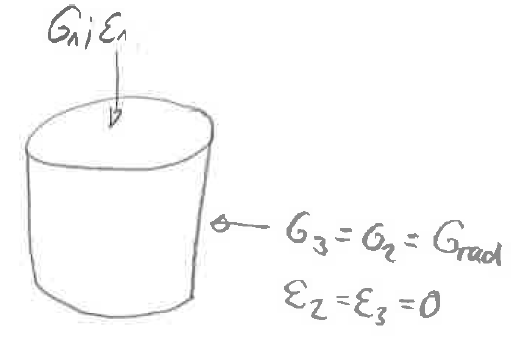
\includegraphics[width=0.5\linewidth]{images/MC1Oed.PNG}
\end{minipage}



\clearpage



\begin{minipage}{0.4\linewidth}
\subsection{Ebenerspannungsraum}
%	\vspace{5cm}
%\textbf{Tau-Sp-Diagramm}
	\begin{align*}
		\tau 		&= c`+ \sigma \cdot tan(\varphi) \\
		\tau		&= b + s`\cdot tan(\beta) \\
		\rightarrow c&= \frac{b`}{cos(\varphi)} \\
		\rightarrow sin(\varphi) &= tan(\beta) \\
	\end{align*}
\end{minipage}
\begin{minipage}{0.5\linewidth}
	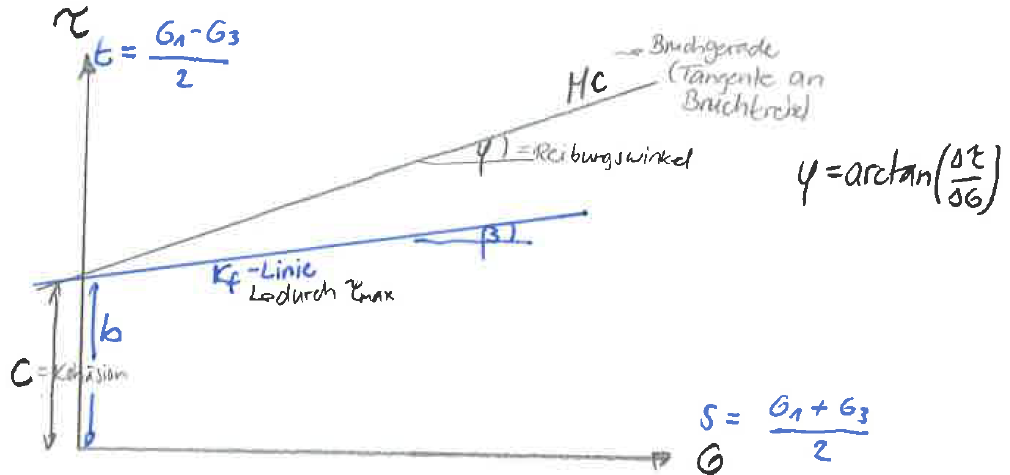
\includegraphics[width=\linewidth]{images/MC2Ebenerspraum.PNG}
\end{minipage}



	
\begin{minipage}{0.6\linewidth}
	\subsection{Dreidimensional}
	\begin{align*}
		q			&= \sigma = M \cdot p + d \\
		M			&= \frac{3 \cdot sin(\varphi)}{\sqrt{3} \cdot cos(\Theta) - sin(\Theta) \cdot sin(\varphi)} \\
					& \rightarrow \Theta = Theta =Winkel der Sp. welche Probe belastet\\
	\end{align*}
\end{minipage}
\begin{minipage}{0.4\linewidth}
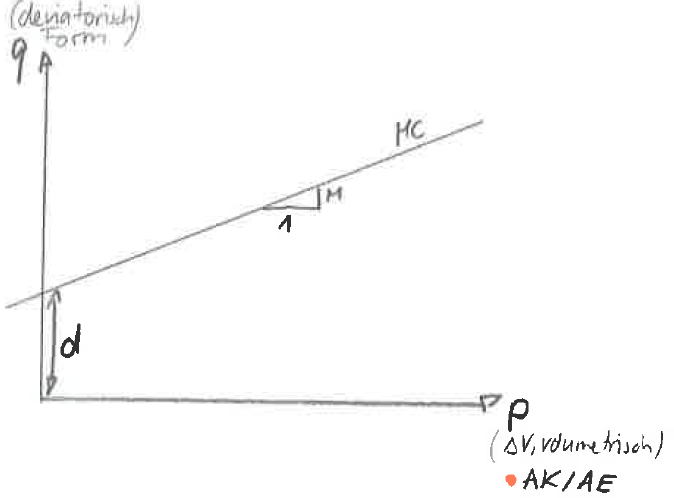
\includegraphics[width=\linewidth]{images/MC33draum.PNG}
\end{minipage}


\begin{minipage}{0.3\linewidth}	
	\subsubsection{Triaxversuch AK}
	\begin{align*}
		M			&= \frac{6 - sin(\varphi)}{3 - sin(\varphi)} \\
		d			&= \frac{6 \cdot c`\cdot cos(\varphi)}{3 - sin(\varphi)} \\
		\Theta		&= 30° = \frac{\pi}{6} \\
	\end{align*}
\end{minipage}
\begin{minipage}{0.5\linewidth}
	\begin{align*}
		\Theta		&= - \frac{\pi}{6}
		\rightarrow \textbf{Kompression}
		&\rightarrow &M_{AK} = \frac{6 \cdot sin(\varphi)}{3 - sin(\varphi)}
		\qquad &d_{AK} = \frac{6 \cdot c`\cdot cos(\varphi)}{3 - sin(\varphi)} \\
		\Theta		&= + \frac{\pi}{6}
		\rightarrow \textbf{Extenssion}
		&\rightarrow &M_{AE} = \frac{- 6 \cdot sin(\varphi)}{3 + sin(\varphi)}
		\qquad &d_{AE} = \frac{- 6 \cdot c`\cdot cos(\varphi)}{3 + sin(\varphi)}
	\end{align*}
\end{minipage}

\begin{minipage}{\linewidth}
	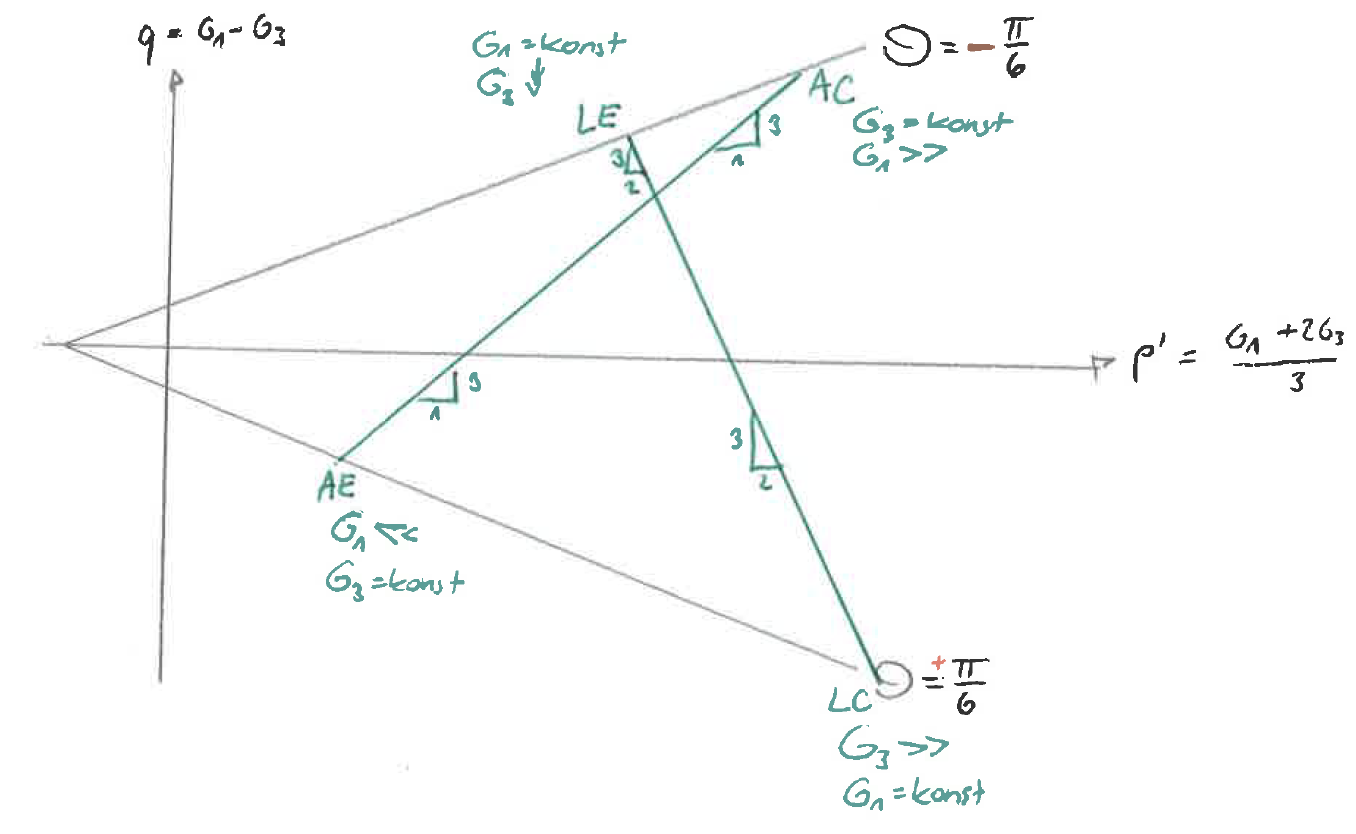
\includegraphics[width=0.8\linewidth]{images/MC4triax.PNG}
\end{minipage}

\clearpage
\end{document}
